\documentclass[11pt]{article}
\usepackage[T1]{fontenc}
\usepackage{lmodern}
\usepackage[margin=0.93in]{geometry}
\usepackage{amsmath,amssymb,amsthm,mathtools}
\usepackage{microtype,booktabs,array,longtable,graphicx}
\usepackage[colorlinks=true,urlcolor=teal!65!black,linkcolor=black]{hyperref}
\usepackage[table]{xcolor}
\usepackage{fancyhdr,enumitem}
\definecolor{ink}{HTML}{172F36}
\definecolor{teal}{HTML}{2F6B69}
\definecolor{muted}{HTML}{5C7775}
\hypersetup{pdftitle={Paper III: Analytic Packet Jets and Release Evidence},pdfauthor={Komorebi P.},pdfsubject={Mathematical supplement with explicitly bounded Lean coverage}}
\pagestyle{fancy}\fancyhf{}\fancyhead[L]{\small\textcolor{teal}{REALIZATION CALCULUS / PAPER III}}\fancyhead[R]{\small\textcolor{muted}{Section 17}}\fancyfoot[C]{\thepage}\setlength{\headheight}{14pt}
\newtheorem{theorem}{Theorem}[section]
\newtheorem{proposition}[theorem]{Proposition}
\newtheorem{corollary}[theorem]{Corollary}
\newtheorem{lemma}[theorem]{Lemma}
\theoremstyle{remark}\newtheorem{remark}[theorem]{Remark}
\newcommand{\X}{\mathsf X}\newcommand{\Y}{\mathsf Y}\newcommand{\Z}{\mathsf Z}
\newcommand{\norm}[1]{\left\lVert#1\right\rVert}
\newcommand{\id}{\mathrm{id}}
\newcommand{\D}{\mathrm D}
\newcommand{\op}{\operatorname}
\setlist[itemize]{itemsep=3pt,topsep=4pt}
\begin{document}
\begin{center}
{\small\bfseries\textcolor{teal}{OPERATION KOMOREBI}}\\[5pt]
{\Large\bfseries Projector Resolved Seed Calculus III}\\[7pt]
{\LARGE\bfseries Analytic Packet Jets and Exact Composition}\\[8pt]
{\large Mathematical and verification supplement}\\[8pt]
{\normalsize Komorebi P. \quad 20 October 2026}\\[9pt]
{\small Private scoped publication edition \quad $\cdot$ \quad Version 1.0.0}
\end{center}
\vspace{6pt}
\noindent\rule{\linewidth}{.8pt}
\vspace{4pt}
This supplement gives full ordinary mathematical arguments for the analytic packet claims of Section 17, identifies a stronger norm bound, and records how the calculation relates to the actual projector ranges. It does \emph{not} assert new Lean kernel verification. The formal algebraic development through Section 16 retains its recorded evidence. The newer Section 17 Lean files are candidates, not accepted proofs.

\section{Two distinct contracts}
Let $\X,\Y,\Z$ be real Banach spaces. A \emph{bounded packet system} on $\X$ is a finite family $P_i\in\mathcal L(\X,\X)$ such that
\begin{equation}\label{eq:proj}
\sum_{i\in I}P_i=\id_{\X},\qquad P_i^2=P_i,\qquad P_iP_j=0\quad(i\ne j).
\end{equation}
Write $\X_i=\op{ran}P_i$ with the subspace norm. Analogously, let $(Q_\gamma)_{\gamma\in J}$ and $(R_\delta)_{\delta\in K}$ be bounded packet systems on $\Y$ and $\Z$.

A weaker family of operators that only satisfies $\sum_iP_i=\id$ yields a useful algebraic expansion, but it need not produce independent coordinates. We keep these statements separate.

\begin{lemma}[Closed ranges and bounded coordinates]\label{lem:closed}
Each $\X_i$ is closed. The maps
\[
A_{\X}(x)=(P_i x)_{i\in I}:\X\longrightarrow\prod_{i\in I}\X_i,
\qquad S_{\X}((z_i)_{i\in I})=\sum_{i\in I}z_i
\]
are inverse bounded linear maps when the finite product carries the maximum norm.
\end{lemma}
\begin{proof}
The identity $\op{ran}P_i=\ker(\id-P_i)$ follows from idempotence. The kernel of a continuous linear map is closed. Both coordinate maps are bounded because the family is finite. Completeness gives $S_{\X}A_{\X}=\id$. If $z_i\in\op{ran}P_i$, then $P_i z_i=z_i$ and $P_j z_i=0$ for $j\ne i$. Thus $A_{\X}S_{\X}=\id$. Moreover,
$\norm{A_{\X}}\le\max_i\norm{P_i}$ and
$\norm{S_{\X}}\le |I|$ whenever $I$ is nonempty. The zero-space case follows from the identities directly.
\end{proof}

\section{Multilinear reconstruction and packet jets}
\begin{theorem}[Completeness is enough for multilinear expansion]\label{thm:reconstruction}
Let $I,J$ be finite. Suppose $\sum_iP_i=\id_{\X}$ and $\sum_\gamma Q_\gamma=\id_{\Y}$, without assuming idempotence or annihilation. Let $B:\X^r\to\Y$ be multilinear. Then, for all $h_1,\ldots,h_r\in\X$,
\begin{equation}\label{eq:recon}
B(h_1,\ldots,h_r)=\sum_{\gamma\in J}\sum_{\alpha\in I^r}
Q_\gamma B(P_{\alpha_1}h_1,\ldots,P_{\alpha_r}h_r).
\end{equation}
The statement includes $r=0$ under the usual empty-product convention.
\end{theorem}
\begin{proof}
For every input, $h_a=\sum_{i\in I}P_i h_a$. Additivity in each slot expands $B$ into the sum over all choices $\alpha\in I^r$. The finite output identity expresses each resulting value as its sum of $Q_\gamma$ components. All exchanges of sums are finite. No property beyond completeness and multilinearity enters the calculation. For $r=0$, the input-index sum has exactly one term, and output completeness still gives the identity.
\end{proof}

\begin{proposition}[Literal continuous range jet]\label{prop:rangejet}
Under \eqref{eq:proj} for the input and output families, let $B:\X^r\to\Y$ be continuous multilinear, $r\ge1$. The formula
\[
J_{\gamma\mid\alpha}B(z_1,\ldots,z_r)
=Q_\gamma B(z_1,\ldots,z_r),\qquad z_a\in\X_{\alpha_a},
\]
defines a continuous multilinear map $\prod_a\X_{\alpha_a}\to\Y_\gamma$ with the actual range as codomain. For $z_a=P_{\alpha_a}h_a$, its image in $\Y$ is the corresponding summand in \eqref{eq:recon}.
\end{proposition}
\begin{proof}
The output lies in $\op{ran}Q_\gamma$ by construction. The subspace inclusions are continuous and isometric. The output projector $Q_\gamma$ and $B$ are continuous. Their composition therefore gives a continuous multilinear map into $\Y$. Since $\Y_\gamma$ carries the induced norm and is closed, viewing this value in $\Y_\gamma$ does not change its norm or continuity. On the projected arguments $P_{\alpha_a}h_a$, the defining expression is precisely the summand in \eqref{eq:recon}.
\end{proof}

\begin{proposition}[A stronger range norm bound]\label{prop:norm}
The literal range jet satisfies
\begin{equation}\label{eq:strong}
\norm{J_{\gamma\mid\alpha}B}\le \norm{Q_\gamma}\,\norm{B}.
\end{equation}
Its ambient extension $\widetilde J=Q_\gamma\circ B\circ(P_{\alpha_1},\ldots,P_{\alpha_r})$ satisfies
\begin{equation}\label{eq:ambient}
\norm{\widetilde J}\le\norm{Q_\gamma}\,\norm{B}\prod_{a=1}^r\norm{P_{\alpha_a}}.
\end{equation}
In particular, the published bound for the range jet with the projector norm product on the right follows from \eqref{eq:strong}.
\end{proposition}
\begin{proof}
For inputs $z_a\in\X_{\alpha_a}$, the induced norms yield
$\norm{Q_\gamma B(z_1,\ldots,z_r)}\le\norm{Q_\gamma}\norm{B}\prod_a\norm{z_a}$, proving \eqref{eq:strong}. Apply additionally $\norm{P_{\alpha_a}h_a}\le\norm{P_{\alpha_a}}\norm{h_a}$ to obtain \eqref{eq:ambient}. If every selected input projector is nonzero, idempotence implies $\norm{P_{\alpha_a}}\ge1$ by evaluating at a unit vector in its range. Then \eqref{eq:strong} implies the weaker published inequality. If any selected input projector is zero, the corresponding input range is the zero space and the positive-order jet is zero. Both sides of the published inequality then vanish. This completes the comparison, including the degenerate case.
\end{proof}

\section{Derivatives, coordinates, and Taylor remainder}
Let $U\subset\X$ be open and $F:U\to\Y$ be $C^m$. For $1\le r\le m$, the Fr\'echet derivative $\D^rF(x)$ is continuous multilinear. Apply Theorem~\ref{thm:reconstruction} to $B=\D^rF(x)$. Thus the actual packet jets recover the entire derivative, without presupposing a separate packet derivative object.

\begin{corollary}[Conjugated derivatives in packet coordinates]\label{cor:conj}
Let $\widehat F=A_{\Y}\circ F\circ S_{\X}$ on the open set $A_{\X}(U)$. Then $\widehat F$ is $C^m$ and
\[
\D^r\widehat F(u)[v_1,\ldots,v_r]
=A_{\Y}\big(\D^rF(S_{\X}u)[S_{\X}v_1,\ldots,S_{\X}v_r]\big).
\]
If $v_a$ is supported only in packet slot $\alpha_a$, let $z_a\in\X_{\alpha_a}$ denote its nonzero coordinate. Then output component $\gamma$ is
\[
J_{\gamma\mid\alpha}(\D^rF(S_{\X}u))[z_1,\ldots,z_r].
\]
\end{corollary}
\begin{proof}
The operators $A_{\Y}$ and $S_{\X}$ are bounded and linear by Lemma~\ref{lem:closed}. Applying the ordinary Fr\'echet chain rule repeatedly, their higher derivatives vanish. Hence the stated formula. The last assertion follows because $S_{\X}$ includes a single supported slot into $\X$ and $A_{\Y}$ applies $Q_\gamma$ in the chosen output slot.
\end{proof}

\begin{theorem}[Packet Taylor identity with integral remainder]\label{thm:taylor}
Let $F:U\to\Y$ be $C^{m+1}$ on an open set containing the closed segment $[x,x+h]$. For $m\ge0$,
\[
Q_\gamma F(x+h)=Q_\gamma F(x)
+\sum_{r=1}^{m}\frac{1}{r!}\sum_{\alpha\in I^r}
J_{\gamma\mid\alpha}(\D^rF(x))
[P_{\alpha_1}h,\ldots,P_{\alpha_r}h]
+Q_\gamma R_{m+1},
\]
where
\[
R_{m+1}=\frac1{m!}\int_0^1(1-t)^m\D^{m+1}F(x+th)[h^{m+1}]\,dt.
\]
If $\norm{\D^{m+1}F(x+th)}\le M$ on the segment, then
\[
\norm{Q_\gamma R_{m+1}}\le\frac{\norm{Q_\gamma}\,M\norm{h}^{m+1}}{(m+1)!}.
\]
\end{theorem}
\begin{proof}
The function $g(t)=F(x+th)$ is a $C^{m+1}$ Banach-valued function on a neighborhood of $[0,1]$. Repeated chain differentiation gives $g^{(r)}(t)=\D^rF(x+th)[h^r]$. Apply the one-dimensional Taylor formula with the Bochner integral remainder. Each $Q_\gamma$ is bounded, so it commutes with the Bochner integral. Expand the finite derivative sum by Theorem~\ref{thm:reconstruction} and take its $\gamma$ component. For the bound use $\norm{Q_\gamma v}\le\norm{Q_\gamma}\norm{v}$, the operator norm of the derivative, and $\int_0^1(1-t)^m\,dt=1/(m+1)$.
\end{proof}

\section{The partition chain rule and packet decorations}
Let $G:\X\to\Y$ and $F:\Y\to\Z$ be $C^n$ on the relevant open sets, with $G$ mapping its domain into the domain of $F$. Write $\Pi_n$ for set partitions of $\{1,\ldots,n\}$.
\begin{theorem}[Fa\`a di Bruno in Banach spaces]\label{thm:faa}
For $n\ge1$,
\[
\D^n(F\circ G)(x)[h_1,\ldots,h_n]
=\sum_{\pi\in\Pi_n}\D^{|\pi|}F(Gx)
\left[\D^{|B|}G(x)[h_i:i\in B]:B\in\pi\right].
\]
The order of blocks is immaterial because Fr\'echet higher derivatives are symmetric.
\end{theorem}
\begin{proof}
For $n=1$ this is the chain rule. Suppose the identity holds at order $n$ and the maps are $C^{n+1}$. Differentiate a summand in direction $h_{n+1}$. Differentiating the outer $\D^{|\pi|}F(Gx)$ produces the same partition with the new singleton block $\{n+1\}$. Differentiating the argument $\D^{|B|}G(x)[h_i:i\in B]$ produces the partition obtained by adjoining $n+1$ to the existing block $B$. Every partition of $\{1,\ldots,n+1\}$ arises in exactly one of these ways, depending on whether $\{n+1\}$ is a singleton. The product and chain rules apply to the bounded multilinear evaluations, and all sums are finite. Induction completes the proof.
\end{proof}

\begin{corollary}[Decorated packet chain rule]\label{cor:decorated}
Fix input labels $\alpha_i$, directions $h_i\in\X_{\alpha_i}$, and an output label $\delta$. For each partition $\pi$ and intermediate label function $\gamma:\pi\to J$, replace the $B$th argument of the outer derivative by $Q_{\gamma(B)}\D^{|B|}G(x)[h_i:i\in B]$. The sum over all such decorations, followed by $R_\delta$, equals the $\delta$ output packet of $\D^n(F\circ G)(x)[h_1,\ldots,h_n]$.
\end{corollary}
\begin{proof}
In every outer argument of Theorem~\ref{thm:faa}, insert the identity on $\Y$ as $\sum_{\gamma\in J}Q_\gamma$. Expand by multilinearity. The output projection $R_\delta$ distributes over the finite sum. Because the directions are already in their actual packet ranges, this is precisely the literal packet-jet expression. No statement assumes that mixed input labels disappear.
\end{proof}

\begin{proposition}[Decorated term count and pruning]\label{prop:count}
If the intermediate family contains $M$ packet labels, the number of formal decorated terms before pruning is
\[
N_{n,M}=\sum_{k=1}^{n}S(n,k)M^k,
\]
where $S(n,k)$ is a Stirling number of the second kind. A decorated summand vanishes if any of its constituent packet jets vanishes. The support of the composed jet is contained in the combinatorially admissible decorated support. Equality of supports need not hold because nonzero terms may cancel.
\end{proposition}
\begin{proof}
There are $S(n,k)$ partitions with $k$ blocks and $M^k$ functions assigning labels to those blocks. The support assertion follows by multilinearity, since a zero argument or a zero outer restricted jet yields a zero summand. The formula is a sum, not a disjoint union of nonzero vectors, so cancellation is allowed. These are statements about formal summands, not claims of computational sparsity for arbitrary coordinate systems.
\end{proof}

\begin{figure}[t]
\centering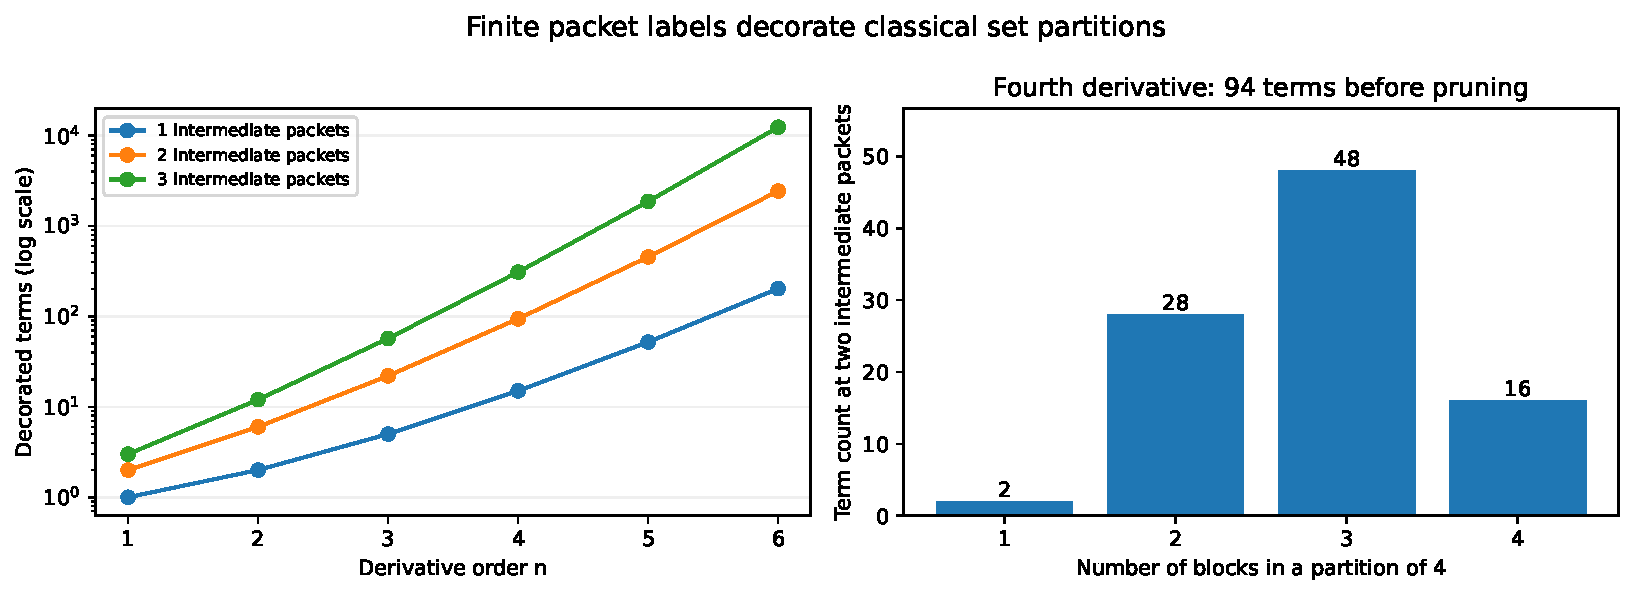
\includegraphics[width=\linewidth]{decorated_partition_terms.pdf}
\caption{The growth of labeled partition terms. At fourth order with two intermediate packet labels, the four block-count contributions are $2$, $28$, $48$, and $16$, totaling $94$. These are exact combinatorial counts, before structural pruning or cancellations.}
\end{figure}

\section{Reproducibility and limitations}
\begin{longtable}{@{}p{.29\linewidth}p{.62\linewidth}@{}}
\toprule
\textbf{Layer}&\textbf{Acceptable inference}\\\midrule\endhead
Section 16 Lean&The recorded 12-module production closure, 558 logical declarations, and 14 separately inventoried runtime helpers remain inherited accepted evidence, not a fresh replay.\\
Section 17 ordinary proofs&The Banach-space identities in this supplement are mathematical arguments, without a current compiler certificate. The range bound \eqref{eq:strong} strengthens the printed proposition.\\
Independent exact checks&Original Section 16 and 17 suites were replayed. New exact polynomial examples verify decorated chain rules through order four and Taylor remainder identities. These do not establish a general theorem.\\
Unaccepted Lean sources&Two Section 17 candidate files are preserved outside the accepted import graph. Neither is counted as compiled.\\
Expanded monograph beyond Section 17&Written proofs and analyses are preserved. Their full correspondence to the formal development has not been demonstrated. The separate October 16 larger declaration count has not been authenticated.\\
Public redistribution&A project-wide license has not been selected. This is a private release package and grants no new redistribution permission.\\
\bottomrule
\end{longtable}

\noindent\textbf{Reading rule.} A valid ordinary proof, an exact computation, a Lean theorem under explicit hypotheses, and an open research construction are separate kinds of evidence. Paper III's release records identify each rather than silently promoting one into another.
\end{document}
